%%%%%%%%%%%%%%%%%%%%%%%%%%%%%%%%%%%%%%%%%%%%%%%%%%%%%%%%%%%%%%%%%%%%%
%% This is a (brief) model paper using the achemso class
%% The document class accepts keyval options, which should include
%% the target journal and optionally the manuscript type. 
%%%%%%%%%%%%%%%%%%%%%%%%%%%%%%%%%%%%%%%%%%%%%%%%%%%%%%%%%%%%%%%%%%%%%
\documentclass[journal=jacsat,manuscript=article]{achemso}

%%%%%%%%%%%%%%%%%%%%%%%%%%%%%%%%%%%%%%%%%%%%%%%%%%%%%%%%%%%%%%%%%%%%%
%% Place any additional packages needed here.  Only include packages
%% which are essential, to avoid problems later. Do NOT use any
%% packages which require e-TeX (for example etoolbox): the e-TeX
%% extensions are not currently available on the ACS conversion
%% servers.
%%%%%%%%%%%%%%%%%%%%%%%%%%%%%%%%%%%%%%%%%%%%%%%%%%%%%%%%%%%%%%%%%%%%%
\usepackage[version=3]{mhchem} % Formula subscripts using \ce{}
\usepackage{csquotes}
\usepackage{lineno}
\usepackage{hyperref}
\usepackage{graphicx}
\usepackage{pdfpages}
\usepackage{tikz}
\usetikzlibrary{arrows.meta, positioning, shadows, shapes}

%\linenumbers
%%% \pagestyle{empty}

%%%%%%%%%%%%%%%%%%%%%%%%%%%%%%%%%%%%%%%%%%%%%%%%%%%%%%%%%%%%%%%%%%%%%
%% If issues arise when submitting your manuscript, you may want to
%% un-comment the next line.  This provides information on the
%% version of every file you have used.
%%%%%%%%%%%%%%%%%%%%%%%%%%%%%%%%%%%%%%%%%%%%%%%%%%%%%%%%%%%%%%%%%%%%%
%%\listfiles

%%%%%%%%%%%%%%%%%%%%%%%%%%%%%%%%%%%%%%%%%%%%%%%%%%%%%%%%%%%%%%%%%%%%%
%% Place any additional macros here.  Please use \newcommand* where
%% possible, and avoid layout-changing macros (which are not used
%% when typesetting).
%%%%%%%%%%%%%%%%%%%%%%%%%%%%%%%%%%%%%%%%%%%%%%%%%%%%%%%%%%%%%%%%%%%%%
\newcommand*\mycommand[1]{\texttt{\emph{#1}}}

%%%%%%%%%%%%%%%%%%%%%%%%%%%%%%%%%%%%%%%%%%%%%%%%%%%%%%%%%%%%%%%%%%%%%
%% Meta-data block
%% ---------------
%% Each author should be given as a separate \author command.
%%
%% Corresponding authors should have an e-mail given after the author
%% name as an \email command. Phone and fax numbers can be given
%% using \phone and \fax, respectively; this information is optional.
%%
%% The affiliation of authors is given after the authors; each
%% \affiliation command applies to all preceding authors not already
%% assigned an affiliation.
%%
%% The affiliation takes an option argument for the short name.  This
%% will typically be something like "University of Somewhere".
%%
%% The \altaffiliation macro should be used for new address, etc.
%% On the other hand, \alsoaffiliation is used on a per author basis
%% when authors are associated with multiple institutions.
%%%%%%%%%%%%%%%%%%%%%%%%%%%%%%%%%%%%%%%%%%%%%%%%%%%%%%%%%%%%%%%%%%%%%
\author{Samuele Giani}
\email{samuele.giani@usz.ch}
\affiliation[USZ]
{Universitätsspital Zürich, Rämistrasse 100, 8091 Zürich, Switzerland}
\author{Cosimo A. De Caro}
\email{cosimo.decaro@mt.com}
\affiliation[MT]
{Mettler-Toledo Technologies GmbH, Heuwinkelstrasse 3, 8606 Nänikon, Switzerland}

%%%%%%%%%%%%%%%%%%%%%%%%%%%%%%%%%%%%%%%%%%%%%%%%%%%%%%%%%%%%%%%%%%%%%
%% The document title should be given as usual. Some journals require
%% a running title from the author: this should be supplied as an
%% optional argument to \title.
%%%%%%%%%%%%%%%%%%%%%%%%%%%%%%%%%%%%%%%%%%%%%%%%%%%%%%%%%%%%%%%%%%%%%
\title[GranTED]
  {SUPPLEMENTARY INFORMATION \newline \phantom{.} \hline \phantom{.} \newline A Green, Reagent-Saving Analytical Strategy for Equivalence Point Determination in Potentiometric Titrations via Gran and Schwartz Linearization \newline \phantom{.} \hline \phantom{.}}

%%%%%%%%%%%%%%%%%%%%%%%%%%%%%%%%%%%%%%%%%%%%%%%%%%%%%%%%%%%%%%%%%%%%%
%% Some journals require a list of abbreviations or keywords to be
%% supplied. These should be set up here, and will be printed after
%% the title and author information, if needed.
%%%%%%%%%%%%%%%%%%%%%%%%%%%%%%%%%%%%%%%%%%%%%%%%%%%%%%%%%%%%%%%%%%%%%
%%% \abbreviations{IR,NMR,UV}
%%% \keywords{SMILES, reaction SMILES, Atom Economy, Green Chemistry, sustainability Metrics, Cheminformatics }

%%%%%%%%%%%%%%%%%%%%%%%%%%%%%%%%%%%%%%%%%%%%%%%%%%%%%%%%%%%%%%%%%%%%%
%% The manuscript does not need to include \maketitle, which is
%% executed automatically.
%%%%%%%%%%%%%%%%%%%%%%%%%%%%%%%%%%%%%%%%%%%%%%%%%%%%%%%%%%%%%%%%%%%%%
\begin{document}
%
\section{Access Links}
Interactive Jupyter Notebooks for \textsf{GranTED} are accessible at \newline
\href{https://mybinder.org/v2/gh/sgiani95/GranTEDGreenChem/HEAD}{\texttt{https://mybinder.org/v2/gh/sgiani95/GranTEDGreenChem/HEAD}}
as well available for individual downloading at the github repository \newline\href{https://github.com/sgiani95/GranTEDGreenChem}{\texttt{https://github.com/sgiani95/GranTEDGreenChem}} 
as *.ipynb files. These notebooks include demonstrations for calculations as shown in the article’s examples.

\section{Detailed Equations}

\subsection*{Derivation of the Gran--Schwartz Linear Form}

\subsubsection*{Strong acid--strong base (Gran 1952)}
Consider the titration of $V_0$ mL of a strong acid (concentration $C_A$) with a strong base (concentration $C_B$). Before the equivalence point the hydrogen-ion concentration is
\begin{equation}
[\ce{H+}] = C_A \frac{V_0}{V_0+V} - C_B \frac{V}{V_0+V}.
\end{equation}
Defining the equivalence volume $V_e$ by $C_A V_0 = C_B V_e$ and treating activity coefficients as constant yields
\begin{equation}
(V_0 + V) \times 10^{-\mathrm{pH}} = k (V_e - V) \label{eq:gran1952}
\end{equation}
where $k$ is a constant. Plotting $(V_0 + V) \times 10^{-\mathrm{pH}}$ versus $V$ gives a straight line intersecting the $V$-axis at $V_e$.

\subsubsection*{Weak systems and Schwartz correction (1987)}
For weak bases (e.g.\ TRIS, $pK_a \approx 8.1$) titrated with strong acid, $[\ce{H+}]$ is no longer negligible in the buffer region. Schwartz showed that a corrected titrant volume
\begin{equation}
v_c = V + \frac{V [\ce{H+}]}{F_t}
\end{equation}
(where $F_t$ is the titrant concentration) leads to the linearised form used in GranTED:
\begin{equation}
(V + k) \times 10^{-\mathrm{pH}} = k' (V_e - V) \label{eq:schwartz}
\end{equation}
(with $k$ and $k'$ containing activity and dilution corrections).

\subsubsection*{Practical implementation in GranTED}
The software plots $(V + k) \times 10^{-\mathrm{pH}}$ versus $V$ for the pre-EQP region and performs linear regression. The $V$-intercept gives $V_e$, while the slope and $R^2$ are used to evaluate the three user-tunable criteria (linearity, uncertainty on $V_e$, and agreement with the full-dataset EQP).

\textbf{References}  
Gran, G. \emph{Acta Chem.\ Scand.}, 1950, \textbf{4}, 559--577.  
Gran, G. \emph{Analyst}, 1952, \textbf{77}, 661--671.  
Schwartz, L.\ M. \emph{J.\ Chem.\ Educ.}, 1987, \textbf{64}, 947--950.

\newpage

\section{Analytical Workflows}

\begin{figure}[htbp]
\centering
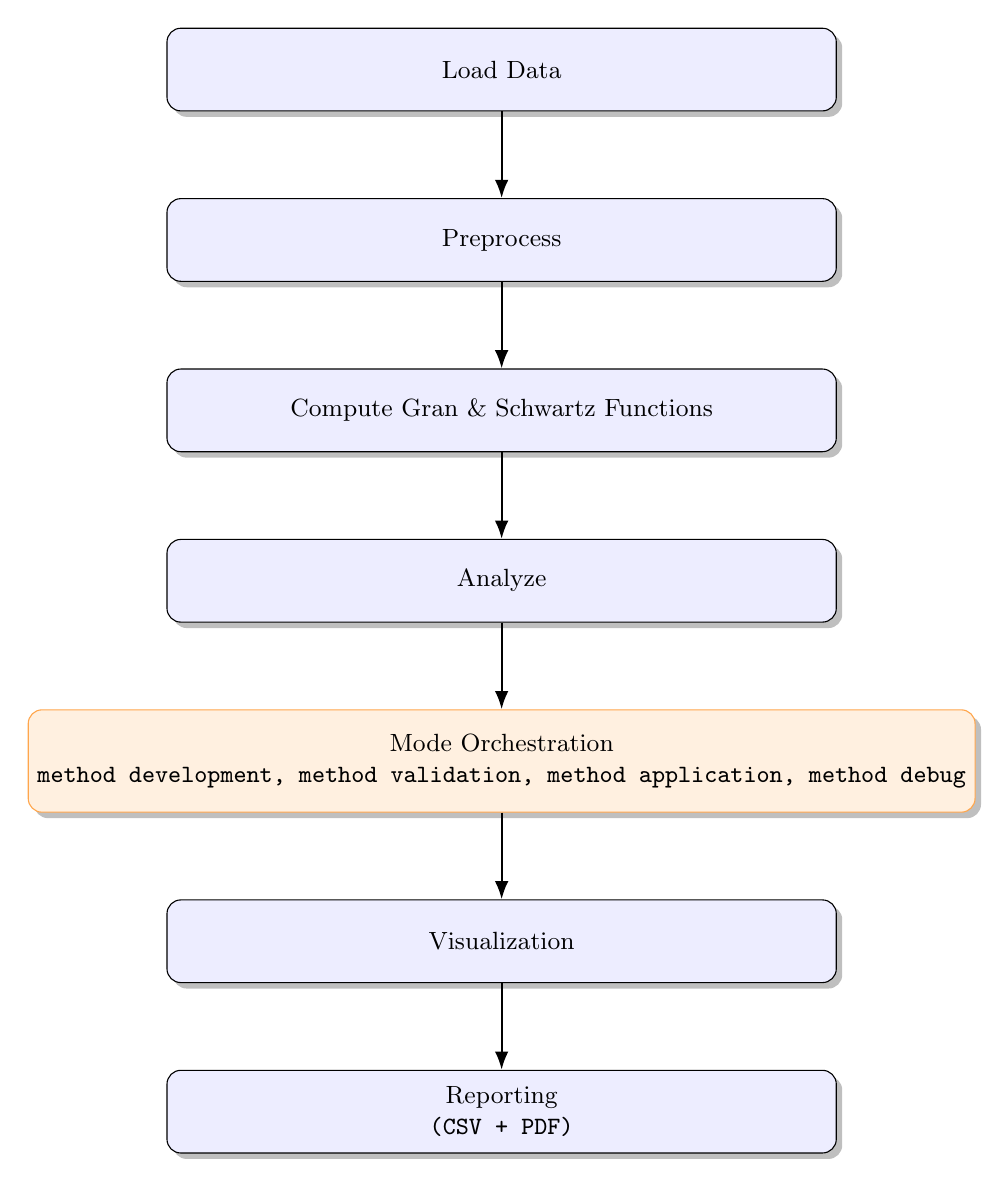
\begin{tikzpicture}[
    node distance=1.1cm,
    box/.style={rectangle, draw, rounded corners=5pt, minimum width=8.5cm, 
                minimum height=1.05cm, align=center, fill=blue!7, drop shadow},
    arrow/.style={-Latex, thick, >=Stealth},
    every node/.style={font=\small}
]

% Main vertical flow
\node[box] (load) at (0,0) {Load Data};
\node[box, below=of load] (preproc) {Preprocess};
\node[box, below=of preproc] (gran) {Compute Gran \& Schwartz Functions};
\node[box, below=of gran] (analyze) {Analyze};

% Mode Orchestration
\node[box, below=of analyze, minimum height=1.3cm, fill=orange!12, draw=orange!70] (modes) {Mode Orchestration \\ \texttt{method development, method validation, method application, method debug}};

% Visualization & Reporting
\node[box, below=of modes] (viz) {Visualization};
\node[box, below=of viz] (report) {Reporting \\ \texttt{(CSV + PDF)}};

% Vertical arrows
\draw[arrow] (load) -- (preproc);
\draw[arrow] (preproc) -- (gran);
\draw[arrow] (gran) -- (analyze);
\draw[arrow] (analyze) -- (modes);
\draw[arrow] (modes) -- (viz);
\draw[arrow] (viz) -- (report);

\end{tikzpicture}
\caption{\textsf{GranTED} workflow}
\label{fig:gran-ted-workflow}
\end{figure}

\newpage

\begin{figure}[htbp]
\centering
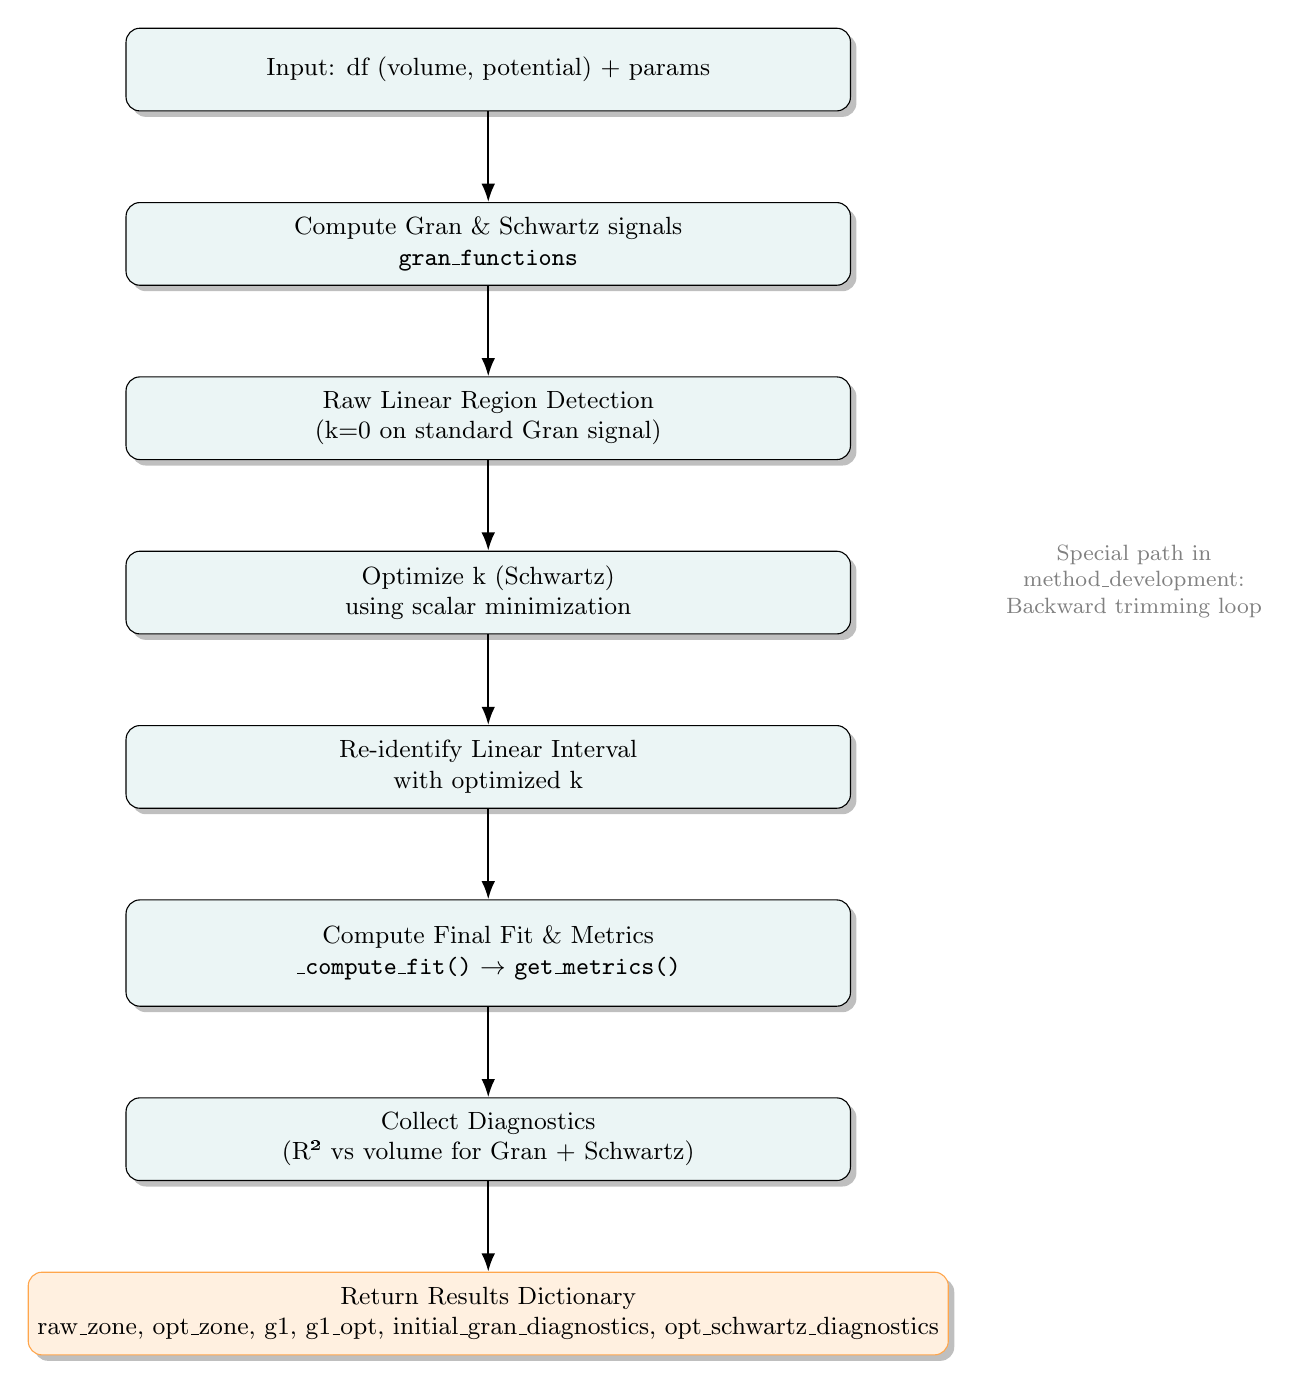
\begin{tikzpicture}[
    node distance=1.15cm,
    box/.style={rectangle, draw, rounded corners=5pt, minimum width=9.2cm, 
                minimum height=1.05cm, align=center, fill=teal!8, drop shadow},
    arrow/.style={-Latex, thick, >=Stealth},
    every node/.style={font=\small}
]

\node[box] (start) at (0,0) {Input: df (volume, potential) + params};

\node[box, below=of start] (granfunc) {Compute Gran \& Schwartz signals \\ \texttt{gran\_functions}};

\node[box, below=of granfunc] (raw) {Raw Linear Region Detection \\ (k=0 on standard Gran signal)};

\node[box, below=of raw] (optk) {Optimize k (Schwartz) \\ using scalar minimization};

\node[box, below=of optk] (reidentify) {Re-identify Linear Interval \\ with optimized k};

\node[box, below=of reidentify, minimum height=1.35cm] (compute) 
    {Compute Final Fit \& Metrics \\ 
     \small \texttt{\_compute\_fit()} $\rightarrow$ \texttt{get\_metrics()} };

\node[box, below=of compute] (diagnostics) {Collect Diagnostics \\ (R² vs volume for Gran + Schwartz)};

\node[box, below=of diagnostics, fill=orange!12, draw=orange!70] (results) 
    {Return Results Dictionary \\ 
     \small raw\_zone, opt\_zone, g1, g1\_opt, initial\_gran\_diagnostics, opt\_schwartz\_diagnostics};

% Arrows
\draw[arrow] (start) -- (granfunc);
\draw[arrow] (granfunc) -- (raw);
\draw[arrow] (raw) -- (optk);
\draw[arrow] (optk) -- (reidentify);
\draw[arrow] (reidentify) -- (compute);
\draw[arrow] (compute) -- (diagnostics);
\draw[arrow] (diagnostics) -- (results);

% Side note for development mode
\node[align=center, font=\footnotesize, text=gray] at (8.2,-6.5) 
    {Special path in \\ method\_development: \\ Backward trimming loop};

\end{tikzpicture}
\caption{Internal workflow of \texttt{analyzer.py} (core analysis pipeline)}
\label{fig:analyzer-workflow}
\end{figure}

\end{document}